\chapter{البيولوجيا البنيوية للبروتينات}\label{ch:b3:structural-biology}

بدأ ماكس بيروتز العمل على بنية الهيموغلوبين عام 1937 ونشرها
عام 1960: اثنتان وعشرون سنة ليرى، \omterm{def:b3:structural-biology:methods}{بتمييز} قدره نصف
نانومتر، كيف تنطوي أربع سلاسل من مئة وخمسين حمضًا أمينيًا
حول أربعة هيمات. وجزيء الهيموغلوبين يطوي نفسه في بضعة
أجزاء من الألف من الثانية. وبين هاتين الحقيقتين يقع موضوع هذا
الفصل: ما شكل البروتين، ولماذا يكون لسلسلة من الأحماض الأمينية
شكل دون آخر، وكيف تجد ذلك الشكل بهذه السرعة بين عدد
فلكي من البدائل، وما الذي يفسد حين لا تجده،
وكيف تُرى الأشكال --- بالأشعة السينية، وبالرنين المغناطيسي، و
بالإلكترونات، واليوم بالحساب --- وكيف يتنقل البروتين بين
الأشكال ليؤدي عمله، والهيموغلوبين بمفتاحه بين صورة متوترة و
أخرى مسترخية هو النموذج لكل بروتين ألوستيري بعده.

\section{ما بنية البروتين}

\begin{definition}[مستويات البنية]\label{def:b3:structural-biology:levels}
\index{بنية ثانوية}\index{لولب ألفا}\index{صفيحة بيتا}\index{بنية ثالثية}\index{نطاق}\index{طية}
\emph{البنية الأولية} هي تسلسل البقايا. و
\emph{البنية الثانوية} هي الانتظام الموضعي المنتظم
للهيكل، تثبته روابط هيدروجينية بين كربونيلات الهيكل
وأميداته: وهي \emph{اللولب $\alpha$}، وهو حلزون أيمن فيه $3.6$
بقية في اللفة، يرتفع \qty{0.15}{nm} لكل بقية (\qty{0.54}{nm}
في اللفة)، ويرتبط كل كربونيل فيه بالأميد الذي يبعد أربع بقايا؛ و
\emph{الصفيحة $\beta$}، وفيها تقع طاقات ممتدة جنبًا إلى جنب،
متوازية أو متعاكسة، مرتبطة بجيرانها، والسلاسل الجانبية
تتناوب فوق الصفيحة وتحتها. و\emph{البنية الثالثية} هي
طية السلسلة كلها في ثلاثة أبعاد؛ والوحدة المرصوصة التي
تنطوي مستقلةً وتضم \numrange{50}{250} بقية داخلها هي \emph{نطاق}،
وترتيب العناصر الثانوية في النطاق هو \emph{طيته}.
و\emph{البنية الرابعية} هي تجمع عدة سلاسل:
كتركيب الهيموغلوبين $\alpha_{2}\beta_{2}$. ونحو \num{1300} طية تفسّر
كل النطاقات المعروفة، وبضع عشرات منها --- طية روسمان، و
برميل TIM، وطية الغلوبولين المناعي --- تفسّر نسبة كبيرة من كل
البروتينات: فالطبيعة تعيد استعمال الطيات وتنوّع تسلسلاتها.
\end{definition}

\begin{omfigure}
\begin{tikzpicture}
\begin{axis}[
  width=6.4cm, height=6.4cm,
  xmin=-180, xmax=180, ymin=-180, ymax=180,
  xlabel={$\phi$ (بالدرجات)}, ylabel={$\psi$ (بالدرجات)},
  xlabel style={font=\small}, ylabel style={font=\small},
  tick label style={font=\scriptsize}, xtick={-180,-90,0,90,180}, ytick={-180,-90,0,90,180},
  axis lines=box, grid=major, grid style={gray!25},
  clip=false,
]
% beta region
\fill[omDef!30] (axis cs:-180,90) rectangle (axis cs:-45,180);
\fill[omDef!30] (axis cs:-180,-180) rectangle (axis cs:-45,-150);
\node[font=\scriptsize, omDef!60!black] at (axis cs:-112,165) {طاقات $\beta$};
% alpha R region
\fill[omThm!30] (axis cs:-160,-70) rectangle (axis cs:-45,0);
\node[font=\scriptsize, omThm!70!black] at (axis cs:-105,-58) {$\alpha$ أيمن};
% alpha L region
\fill[omMeth!30] (axis cs:45,0) rectangle (axis cs:100,80);
\node[font=\scriptsize, omMeth!60!black, align=center] at (axis cs:72,40) {أيسر};
\addplot[only marks, mark=*, mark size=1pt, black] coordinates {(-57,-47)};
\node[font=\scriptsize, anchor=south west] at (axis cs:-52,-44) {$\alpha$: $(-57,-47)$};
\addplot[only marks, mark=*, mark size=1pt, black] coordinates {(-139,135)};
\node[font=\scriptsize, anchor=west] at (axis cs:-134,135) {$\beta$ متعاكسة};
\end{axis}
\node[align=left, font=\scriptsize, anchor=west] at (7.0,3.0) {زاويتا الالتواء في هيكل كل\\بقية، $\phi$ (حول N--C$_\alpha$) و$\psi$ (حول\\C$_\alpha$--C)، يحصرهما التصادم الفراغي\\في المناطق الملونة. فاللولب يضع كل\\بقية عند نقطة واحدة؛ والطاق قرب أخرى.\\والغليسين، بلا سلسلة جانبية، يبلغ أبعد؛\\والبرولين، بحلقته، مثبت قرب $\phi = -60$.};
\end{tikzpicture}

{\small مخطط راماتشاندران. المناطق المظللة هي التوليفات
المسموح بها فراغيًا لزاويتي الهيكل $\phi$ وَ$\psi$؛ ويوافق
اللولب $\alpha$ الأيمن والطاق $\beta$ كلٌّ منهما منطقةً
صغيرة، وتقع معظم بقايا البروتين المطوي في إحداهما.}
\end{omfigure}

\begin{proposition}[ما الذي يمسك الطية]\label{prop:b3:structural-biology:forces}
\index{الأثر الكاره للماء}\index{ثبات هامشي}
يثبّت البروتينَ المطوي \emph{\omterm{prop:b3:structural-biology:forces}{الأثر الكاره للماء}} ---
أي دفن السلاسل الجانبية غير القطبية في لبّ بعيد عن الماء، وهو يحرر
جزيئات الماء التي كانت لتنتظم حولها --- كما تثبّته
الروابط الهيدروجينية في \omterm{def:b3:structural-biology:levels}{البنية الثانوية} وفي الزمر القطبية
المدفونة، وتراصّ فان دير فالس للبّ في كثافة بلورة، و
جسور ملحية عارضة، وفي البروتينات المفرَزة روابط ثنائية
الكبريت. \omterm{prop:b3:structural-biology:forces}{والأثر الكاره للماء} يوفر معظم الدفع؛ أما الروابط
الهيدروجينية فتدفع ثمن نفسها في معظمها (فالهيكل المرتبط بالماء في
الحالة غير المطوية يرتبط بنفسه في المطوية) وتملي بدل ذلك
\emph{أيّ} \omterm{def:b3:structural-biology:levels}{طية}. والطاقة الحرة الصافية للطي صغيرة،
$\Delta G \approx -20$ إلى \qty{-60}{kJ/mol} --- أي قوة
حفنة من الروابط الهيدروجينية لجزيء فيه مئات منها --- لأن
فقد الإنتروبيا الانتظامية عند الطي يكاد يلغي كسب
الإنثالبيا. فالبروتينات \emph{ثابتة ثباتًا هامشيًا}: فبضع درجات، أو
تغير في pH، أو طفرة واحدة في اللب تستطيع أن تفتلها، وهذه
الهامشية هي ما يتيح لها الحركة.
\end{proposition}

\begin{proof}[شواهد]
فتل أنفينسن (1961) الريبونوكلياز~A باليوريا وعامل مرجع،
فكسر روابطه الكبريتية الأربع وأتلف فاعليته؛ وعند إزالة
الاثنين، أعاد الإنزيم طيّ نفسه، وأعاد تكوين الأربعة الصحيحة من بين $105$
ازدواجات كبريتية ممكنة، واستعاد فاعليته كاملةً. فلا قالب،
ولا إنزيم، ولا معلومة سوى التسلسل كانت حاضرة: فالبنية
الأصلية هي أثبت الحالات ترموديناميكيًا مما تبلغه
السلسلة، والتسلسل يشفّرها. وإعادة أكسدة الروابط الكبريتية بينما
كانت السلسلة في اليوريا أعطت خليطًا مشوّشًا فاعليته \qty{1}{\%}،
ثم انفكّ تشويشه إلى الصورة الأصلية حين أُتيح له
الطي: فالسلسلة تجد الأصغرية بنفسها.
\end{proof}

\section{كيف تجد السلسلة طيتها}

\begin{theorem}[مفارقة ليفينثال]\label{thm:b3:structural-biology:levinthal}
\index{مفارقة ليفينثال}\index{قمع الطي}
لو استطاعت كل بقية من بقايا البروتين البالغة $n$ أن تتخذ $k$
انتظامًا هيكليًا استقلالًا، لكان للسلسلة $k^{n}$
انتظام. وعند $k = 3$ وَ$n = 100$ يكون ذلك $3^{100} \approx
5\times 10^{47}$؛ ومعاينتها بواحد في كل بيكوثانية ($10^{12}$ في
الثانية) تستغرق $5\times 10^{35}$ ثانية، أي نحو $10^{28}$ سنة.
والبروتينات بهذا الحجم تنطوي في أجزاء من الألف من الثانية إلى ثوانٍ. فالطي
إذن ليس بحثًا عشوائيًا في الانتظامات: فسطح الطاقة
\emph{قمع}، يكون فيه كل انتظام جزئي تقريبًا
منحازًا نحو الحالة الأصلية، وتنزل السلسلة بحركات
موضعية كل منها هابط في المتوسط.
\end{theorem}
\begin{proof}
العدّ هو مبدأ الضرب؛ والزمن هو العدّ
مقسومًا على معدل المعاينة، $5\times 10^{47}/10^{12} = 5\times
10^{35}$ ثانية، والسنة $3\times 10^{7}$ ثانية. والنتيجة هي
عكس النقيض: فبحث عشوائي بهذا الحجم مستحيل في
الزمن المرصود، فالبحث إذن ليس عشوائيًا. والذي يجعله غير عشوائي
أن التآثر الذي ينعقد في جزء من السلسلة يدوم بينما
تنعقد سواه (فالانهيار الكاره للماء وتكوّن اللوالب يقعان في
ميكروثوانٍ ويقلّصان الفضاء المطلوب مسحه)، وأن البنى الصحيحة
جزئيًا أخفض طاقةً في المتوسط من الخاطئة، فيكون
النزول موجَّهًا --- أي قمعًا لا ملعب غولف فيه
حفرة واحدة.
\end{proof}

\begin{omfigure}
\begin{tikzpicture}[every node/.style={font=\scriptsize}, >=stealth]
  % funnel outline
  \draw[very thick, omDef] (-4,3) .. controls (-3.2,1.5) and (-1.2,0.2) .. (-0.35,-1.2) -- (-0.35,-1.6);
  \draw[very thick, omDef] (4,3) .. controls (3.2,1.5) and (1.2,0.2) .. (0.35,-1.2) -- (0.35,-1.6);
  \draw[very thick, omDef] (-0.35,-1.6) -- (0.35,-1.6);
  % rugged inner lines
  \draw[omDef!60, thick] (-3.3,2.6) .. controls (-2.9,2.2) and (-2.6,2.6) .. (-2.2,2.0) .. controls (-1.9,1.5) and (-1.7,1.9) .. (-1.4,1.2) .. controls (-1.1,0.7) and (-0.9,0.9) .. (-0.6,0.2);
  \draw[omDef!60, thick] (3.3,2.6) .. controls (2.9,2.1) and (2.5,2.5) .. (2.1,1.8) .. controls (1.8,1.3) and (1.5,1.6) .. (1.2,1.0) .. controls (1.0,0.6) and (0.8,0.8) .. (0.6,0.2);
  % axes
  \draw[->] (-5.9,-1.8) -- (-5.9,3.2) node[above, align=center] {الطاقة\\الحرة};
  \draw[<->] (-3.9,3.85) -- (3.9,3.85) node[midway, above] {الإنتروبيا الانتظامية (سعة المجموعة)};
  % labels
  \node[above] at (0,3.05) {سلسلة غير مطوية: انتظامات كثيرة، وطاقة عالية};
  \node[right, align=left] at (3.3,1.4) {مصائد موضعية: وسائط\\مطوية جزئيًا خطأً};
  \node[left, align=right] at (-3.3,1.4) {انهيار سريع وبنية\\ثانوية};
  \node[below] at (0,-1.7) {الحالة الأصلية: انتظام واحد، وأخفض طاقة};
  \draw[->, thick, omThm] (-2.8,2.4) .. controls (-2.0,1.2) and (-0.8,0.5) .. (-0.15,-1.3);
  \node[omThm, left] at (-1.5,-0.5) {مسار طي};
\end{tikzpicture}

{\small \omterm{thm:b3:structural-biology:levinthal}{قمع الطي}. تهبط الطاقة الحرة ويتقلص عدد
الانتظامات المتاحة كلما اقتربت السلسلة من الحالة
الأصلية؛ والجدران وعرة، فقد تُحبس السلسلة في وسيط مطوي
جزئيًا خطأً، لكن الميل العام يحملها نزولًا في
أجزاء من الألف من الثانية.}
\end{omfigure}

\begin{definition}[البروتينات المرافقة]\label{def:b3:structural-biology:chaperones}
\index{بروتين مرافق}\index{Hsp70}\index{مرافقين}\index{GroEL}
\emph{البروتين المرافق الجزيئي} بروتين يعين غيره على
الطي من غير أن يصير جزءًا منه ومن غير أن يمده بمعلومة عن
\omterm{def:b3:structural-biology:levels}{الطية}: فهو يمنع التكتل الذي ينافس الطي في
الهيولى المزدحمة. و\emph{Hsp70} يرتبط بالقطع الكارهة للماء المكشوفة
من السلاسل الوليدة أو غير المطوية، ويطلقها عند حلمهة ATP لمحاولة
أخرى؛ و\emph{المرافقين} GroEL (وهو Hsp60 في المتقدرات،
وTRiC في هيولى حقيقيات النوى) برميل مزدوج من أربع عشرة وحدة
يضم تجويفه المركزي، المغطى بالبروتين GroES، سلسلة واحدة تصل إلى
\qty{60}{kDa} منعزلةً نحو عشر ثوانٍ --- أي قفص أنفينسن
--- ثم يقذفها مطويةً كانت أو لا، لتحاول مرة أخرى. ونحو عُشر
البروتينات البكتيرية المصنوعة حديثًا يمر بالمرافقين GroEL، والخلية التي
تُغرق مرافقاتها --- بالحرارة، ولهذا كان معظمها
\emph{بروتينات الصدمة الحرارية} التي يحرضها ارتفاع الحرارة --- تمتلئ
بالتكتلات.
\end{definition}

\begin{definition}[النشواني]\label{def:b3:structural-biology:amyloid}
\index{نشواني}\index{تصالب بيتا}\index{بريون}\index{مرض سوء الطي}
\emph{النشواني} تكتل منتظم من البروتين تتراص فيه السلاسل
في ليفات غير متفرعة عرضها \qtyrange{5}{10}{nm}، وتسير طاقات
كل سلسلة عمودية على محور الليف ومرتبطة هيدروجينيًا
بطاقات السلسلة التالية --- وهي بنية \emph{التصالب $\beta$}،
وهي نفسها أيًا كان البروتين. ويكاد كل بروتين يستطيع تكوينها في
شروط مزعزعة؛ وفي \emph{أمراض سوء الطي} تفعل ذلك بروتينات
بعينها في الجسم: النشواني $\beta$ وتاو في داء
ألزهايمر، و$\alpha$-سينوكلئين في داء باركنسون، والهنتنغتين، والترانستيريتين،
والنشواني الجزيري في السكري من النمط~2. و\emph{البريون} نشواني
ينتشر: فالصورة السيئة الطي من البروتين البريوني PrP تحوّل
الصورة السوية عند التماس إلى مزيد من نفسها، فلا تحمل ``العدوى''
حمضًا نوويًا بل شكلًا فقط --- وهي آلية السكرابي،
واعتلال الدماغ الإسفنجي البقري، وداء كروتزفيلد--ياكوب،
أثبتها بروسينر منذ عام 1982 في وجه مقاومة طويلة.
\end{definition}

\begin{omfigure}
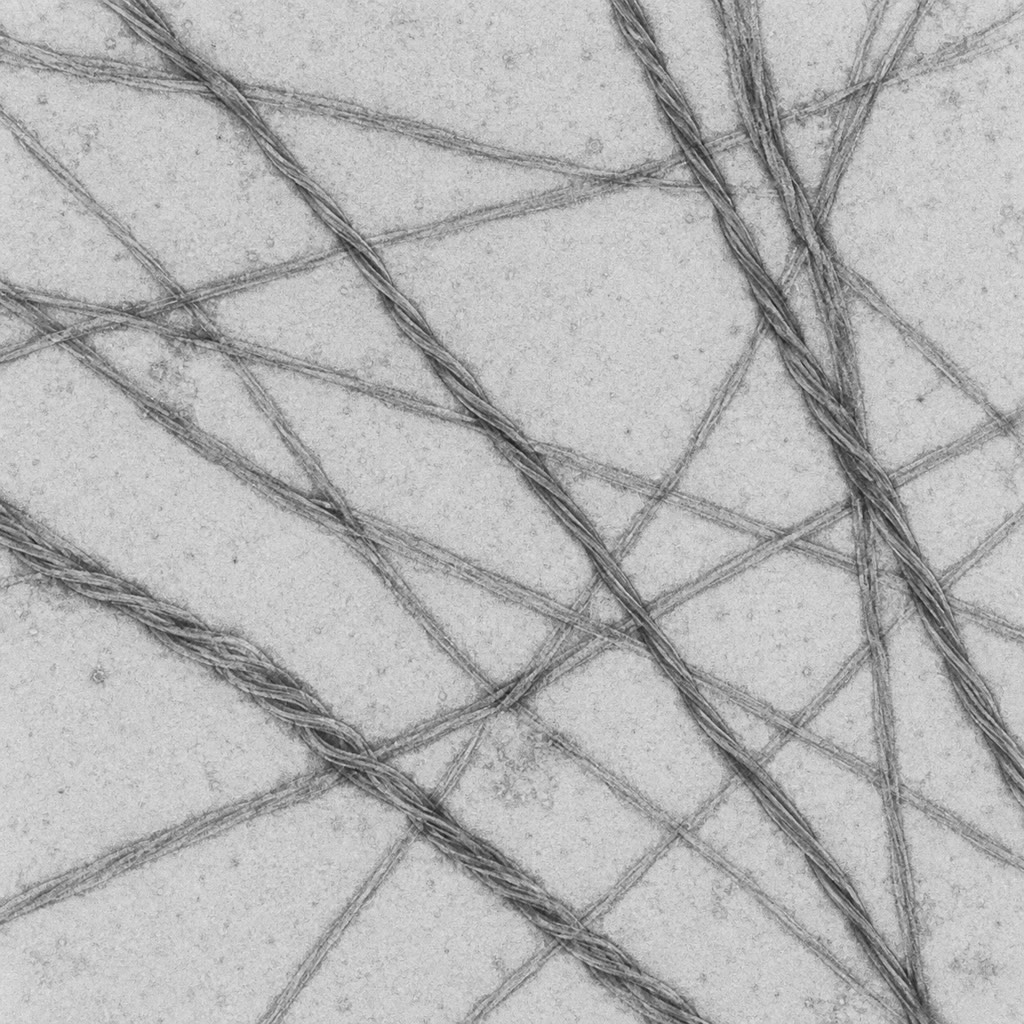
\includegraphics[width=0.36\linewidth]{images/book5/ai/b5-07-amyloid-fibrils.jpg}\hspace{0.04\linewidth}
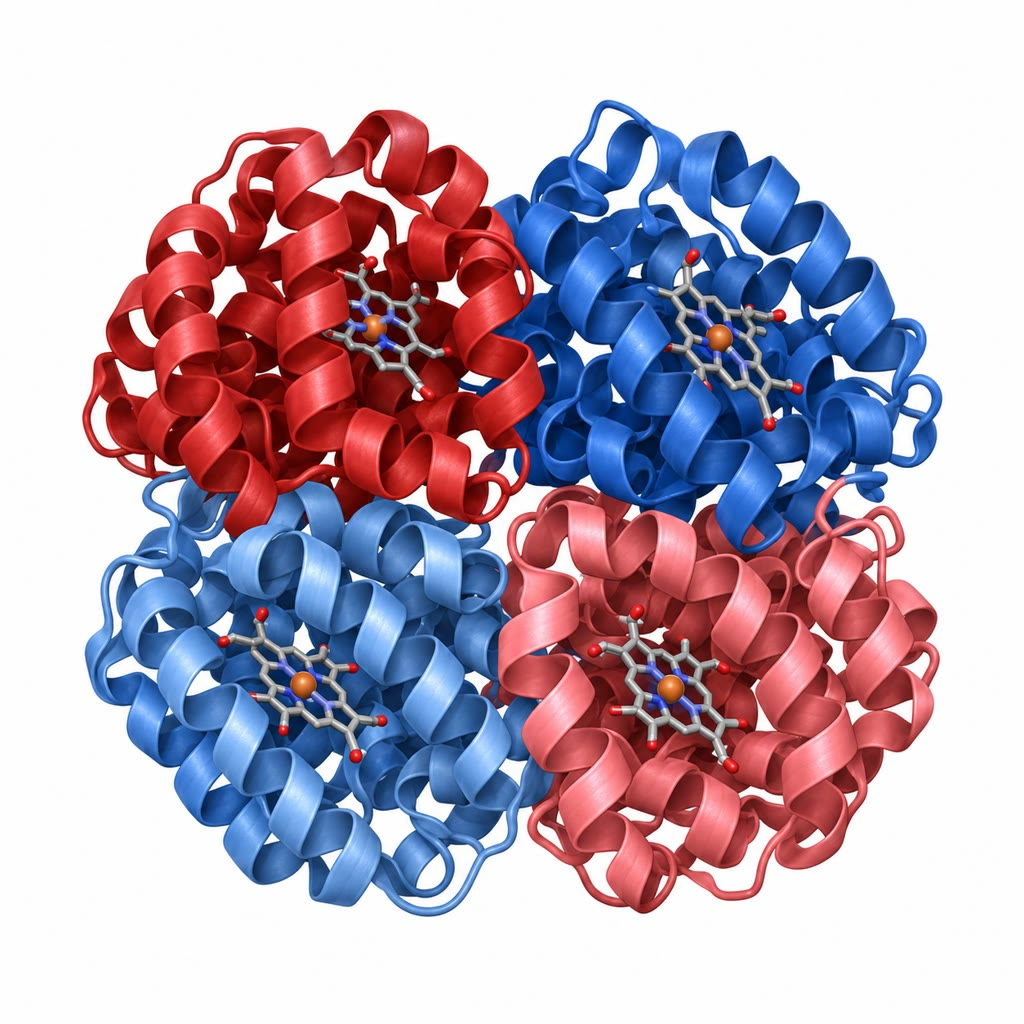
\includegraphics[width=0.36\linewidth]{images/book5/ai/b5-07-haemoglobin-model.jpg}

{\small يسارًا: ليفات نشوانية في المجهر الإلكتروني --- مستقيمة،
غير متفرعة، ملتوية أحيانًا، ومتشابهة بنيويًا أيًا كان البروتين
الذي صُنعت منه. يمينًا: رباعي الهيموغلوبين، سلسلتان $\alpha$ وسلسلتان
$\beta$، تحتضن كل منها هيمًا.}
\end{omfigure}

\section{رؤية بروتين}

\begin{definition}[الطرائق البنيوية]\label{def:b3:structural-biology:methods}
\index{حيود الأشعة السينية}\index{مطيافية الرنين المغناطيسي النووي}\index{مجهر إلكتروني مبرَّد}\index{تمييز}
\emph{حيود الأشعة السينية} ينمّي بلورة من البروتين، ويعرّضها
لحزمة من الأشعة السينية ويسجل نمط الحيود؛ فتعطي
مواضع البقع الشبيكةَ، وتعطي شدّاتها، متى استُعيدت
أطوار الأمواج، الكثافةَ الإلكترونية لخلية
الوحدة، وفيها تُبنى السلسلة. و\emph{الرنين المغناطيسي
النووي} (NMR) يقيس، في المحلول، الاقترانات بين
أنوية الذرات المتقاربة في الفراغ، وتُحسب منها المسافات ومن ثم
بنية؛ وهو يصلح لبروتينات دون نحو \qty{40}{kDa}
ويبلّغ عن حركاتها. و\emph{المجهر الإلكتروني المبرَّد} يصوّر
آلافًا إلى ملايين من الجزيئات المفردة مجمَّدة في غشاء رقيق من
جليد زجاجي، كل منها في اتجاه عشوائي، ويعيد بناء
الكثافة الثلاثية الأبعاد بجمعها؛ ومنذ الكواشف الإلكترونية
المباشرة (2013) صار يبلغ التمييز الذري ولا يحتاج إلى بلورة،
فصارت المعقّدات الكبيرة والبروتينات الغشائية والتجمعات المرنة التي
لم تتبلور قط تُحلّ اليوم روتينيًا. و\emph{تمييز}
البنية هو أصغر مباعدة ينفصل عندها معلمان:
فعند \qty{0.35}{nm} يوضع الهيكل والسلاسل الجانبية الكبيرة، وعند
\qty{0.2}{nm} كل ذرة، وعند \qty{0.1}{nm} الهيدروجينات.
\end{definition}

\begin{proof}[شواهد]
حصل كندرو (1958) على أول بنية لبروتين، وهي ميوغلوبين
حوت العنبر، عند \qty{0.6}{nm} --- سجق غير منتظم على غير توقع،
``أعقد وأقل تناظرًا مما تنبأ به أحد''
--- ثم عند \qty{0.2}{nm} عام 1960، حين رُئيت لأول مرة لوالب $\alpha$ التي
كان باولنغ قد اقترحها من بناء النماذج عام 1951.
وحلّ بيروتز (1960) الهيموغلوبين عند \qty{0.55}{nm} بطريقة
الذرة الثقيلة التي ابتكرها للحصول على الأطوار: فذرات الزئبق
الملتصقة بالبروتين تغيّر الشدات على نحو يكشف
المعلومة الناقصة. وبمقارنة الصورتين المؤكسجة وغير المؤكسجة
(1970) رأى الوحدات تدور بعضها على بعض بمقدار
\qty{15}{\degree} عند ارتباط الأكسجين، وهو أول انتقال ألوستيري
رُصد على المقياس الذري.
\end{proof}

\begin{omfigure}
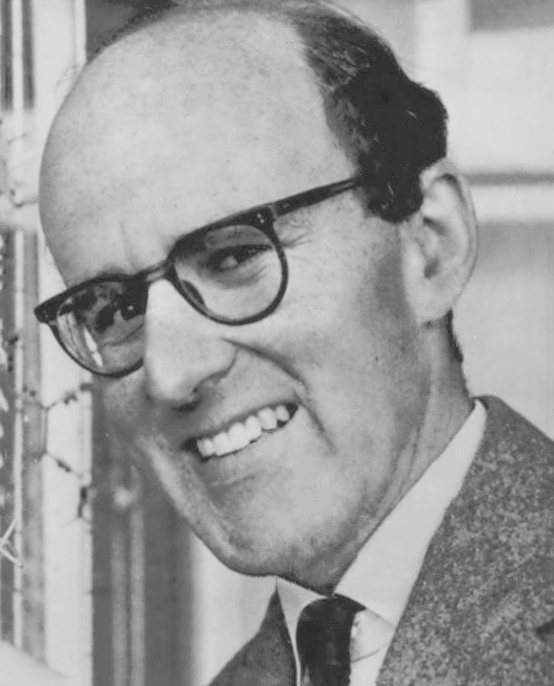
\includegraphics[width=0.30\linewidth]{images/book5/perutz.jpg}\hspace{0.04\linewidth}
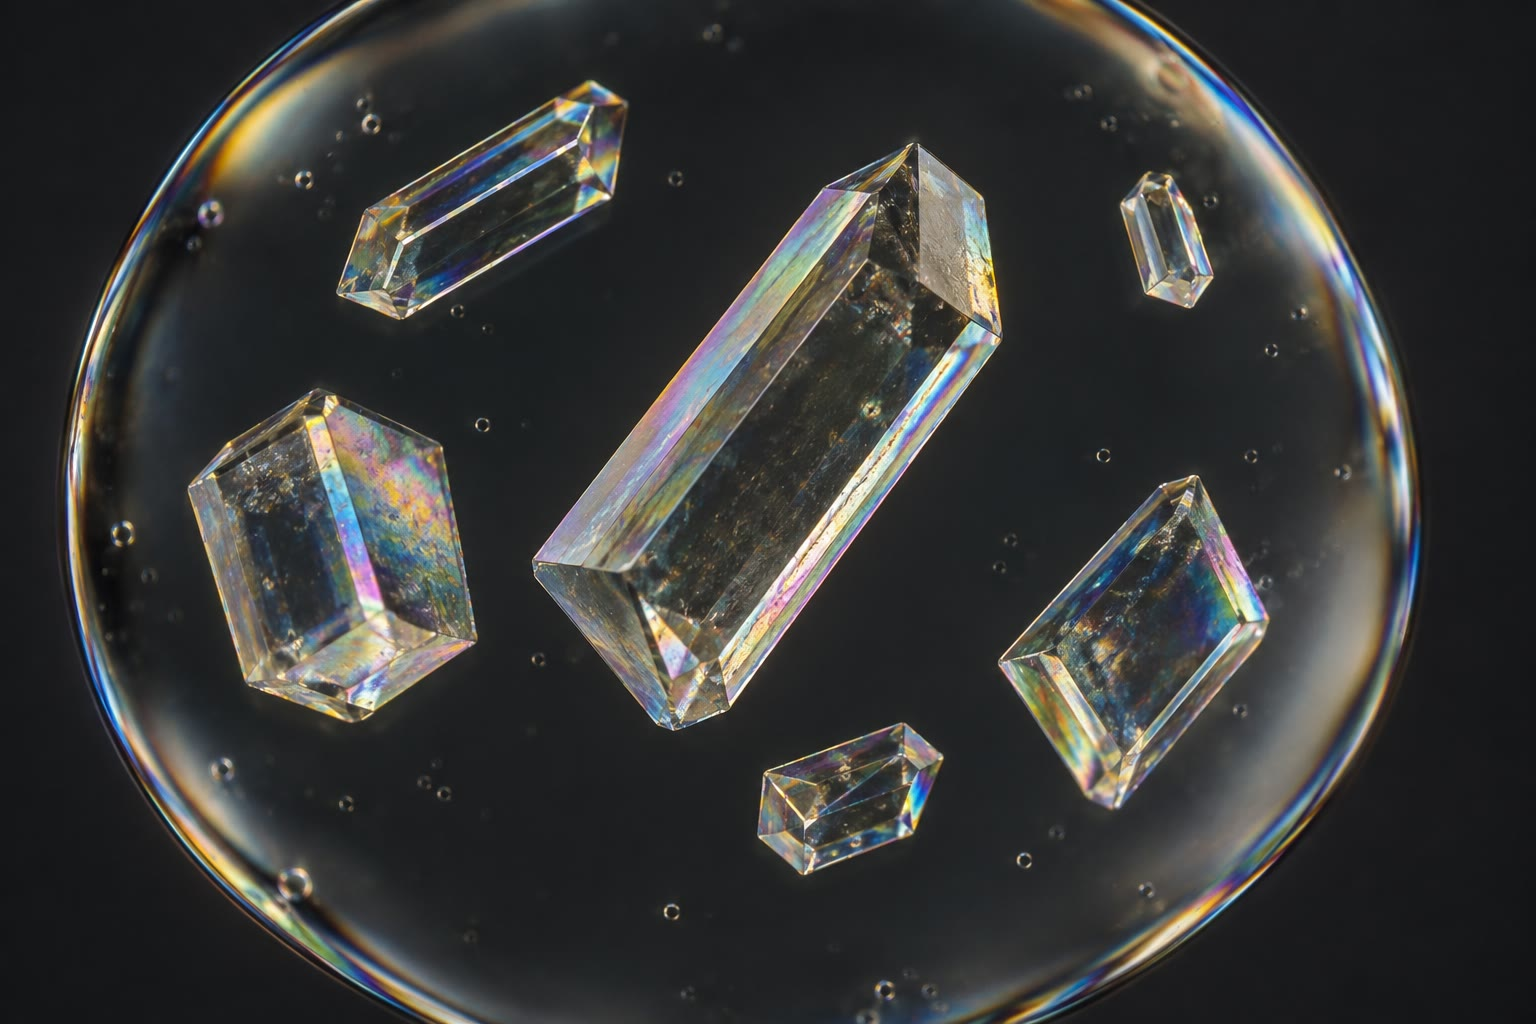
\includegraphics[width=0.30\linewidth]{images/book5/ai/b5-07-protein-crystals.jpg}\hspace{0.04\linewidth}
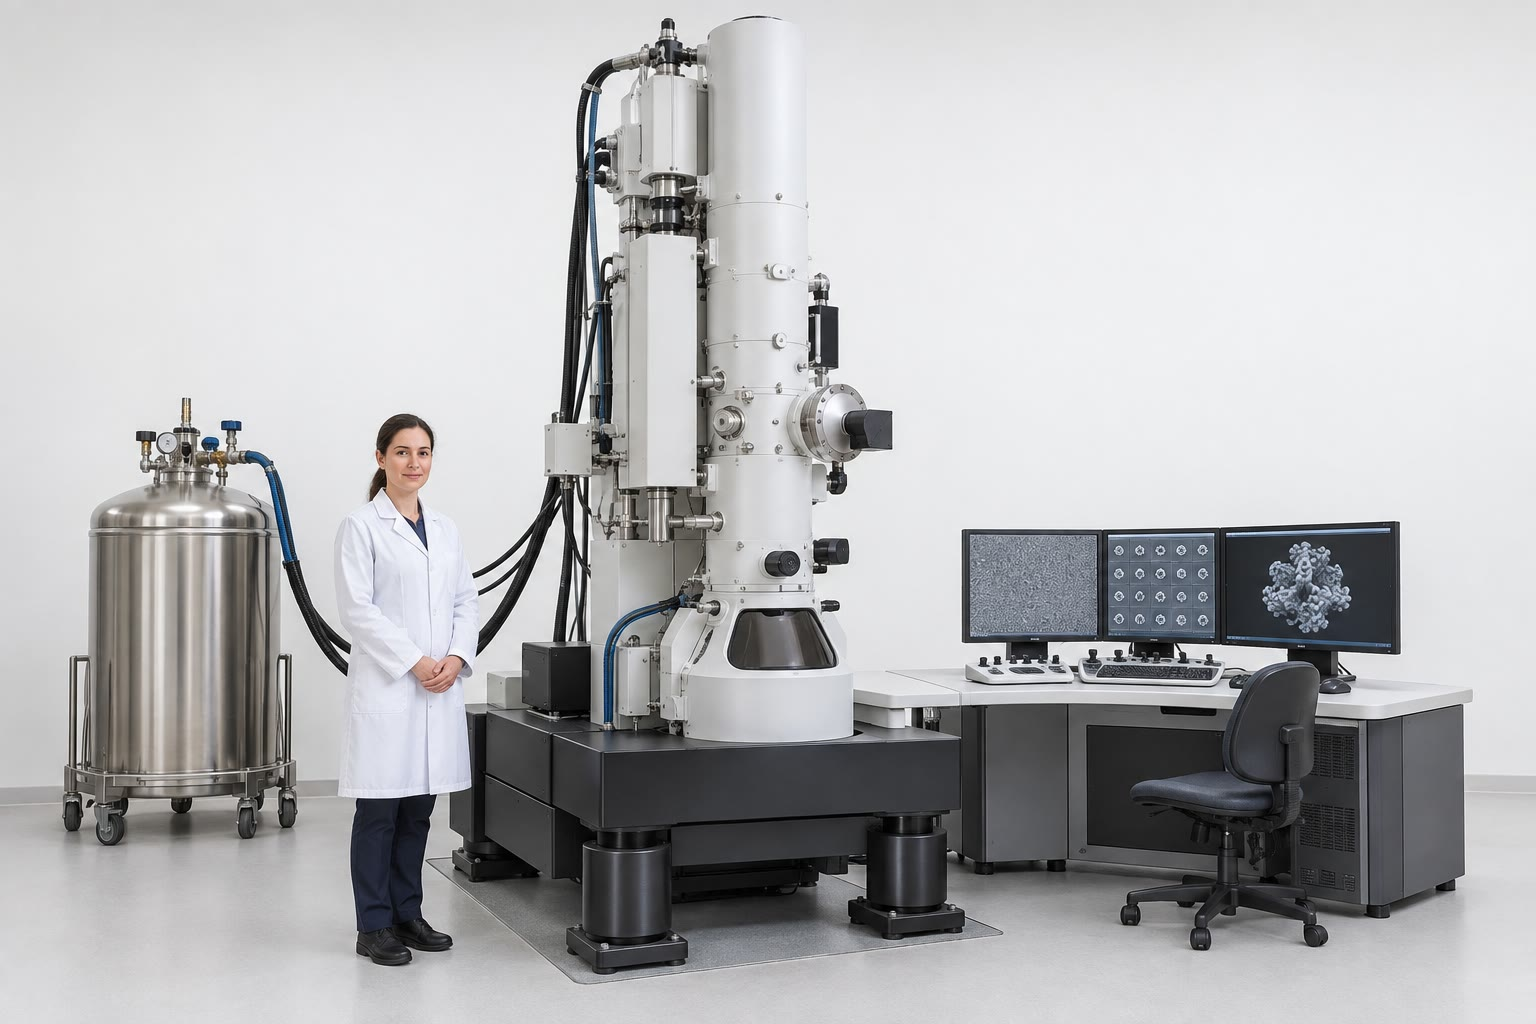
\includegraphics[width=0.30\linewidth]{images/book5/ai/b5-07-cryo-em.jpg}

{\small ماكس بيروتز عام 1962، وهي سنة نيله جائزة نوبل عن
بنية الهيموغلوبين (أسوشيتد برس، ملكية عامة). وفي الوسط:
بلورات بروتين في قطرة معلقة، وهي نقطة بدء
علم البلورات. يمينًا: \omterm{def:b3:structural-biology:methods}{مجهر إلكتروني مبرَّد}، وهو الجهاز
الذي جعل البلورات غير ضرورية.}
\end{omfigure}

\begin{method}[حل بنية بحيود الأشعة السينية]\label{met:b3:structural-biology:crystallography}
\index{قانون براغ}\index{مسألة الطور}
(1) نقّ ميليغرامات من البروتين وافحص مئات الشروط
(المرسّب، وpH، والملح) بحثًا عن بلورات؛ (2) جمّد بلورة تجميدًا خاطفًا
واجمع صور الحيود في مسرّع تزامني وهي تدور في الحزمة؛
(3) فهرس البقع للحصول على خلية الوحدة والتناظر؛ وأكبر
زاوية تُرى عندها بقع تحدد \omterm{def:b3:structural-biology:methods}{التمييز} \omterm{met:b3:structural-biology:crystallography}{بقانون براغ}، $d =
\lambda/(2\sin\theta)$؛ (4) حلّ \emph{\omterm{met:b3:structural-biology:crystallography}{مسألة الطور}} ---
فالكاشف يسجل الشدات لا الأطوار --- بالذرات الثقيلة، أو
بالاستطارة الشاذة للسيلينيوم في السيلينوميثيونين، أو، لبروتين
شبيه ببروتين معروف، بالإبدال الجزيئي، بوضع النموذج
المعروف في الخلية؛ (5) احسب الكثافة الإلكترونية، وابنِ السلسلة
فيها ونقّح النموذج في مواجهة المعطيات حتى يصغر التباين
(العامل $R$)؛ (6) تحقق: من الهندسة، ومن شواذ راماتشاندران،
ومن الملاءمة لمعطيات لم يُنقَّح النموذج في مواجهتها.
\end{method}

\begin{omfigure}
\begin{tikzpicture}[every node/.style={font=\scriptsize}, >=stealth]
  % crystal
  \draw[thick, fill=omDef!20] (0,0) -- (1.4,0) -- (1.9,0.6) -- (0.5,0.6) -- cycle; \draw[thick, fill=omDef!30] (0,0) -- (0.5,0.6) -- (0.5,1.6) -- (0,1.0) -- cycle; \draw[thick, fill=omDef!25] (0.5,0.6) -- (1.9,0.6) -- (1.9,1.6) -- (0.5,1.6) -- cycle;
  \node[below] at (0.95,-0.1) {بلورة: $10^{12}$ جزيء في اصطفاف};
  % beam
  \draw[->, very thick, omThm] (-2.2,0.9) -- (-0.1,0.9); \node[above] at (-1.2,0.95) {أشعة سينية، $\lambda \approx \qty{0.1}{nm}$};
  % diffracted beams
  \foreach \a in {-25,-12,5,18,30} \draw[->, omThm, thick] (1.9,0.9) -- ++(\a:3.2);
  % detector
  \draw[thick] (5.2,-1.2) rectangle (5.6,3.0); \node[right, align=left] at (5.7,2.6) {الكاشف: بقع عند\\زوايا $\theta$، وشدّاتها\\$I$};
  \foreach \y in {-0.6,-0.1,0.6,1.2,1.9,2.4} \fill[black] (5.4,\y) circle (0.06);
  % arrow to density
  \draw[->, very thick] (7.4,0.9) -- (8.6,0.9) node[midway, above, align=center] {استُعيدت\\الأطوار};
  \node[right, align=left] at (8.7,1.4) {الكثافة الإلكترونية};
  \draw[omDef, thick] (8.8,0.4) .. controls (9.1,1.1) and (9.5,0.2) .. (9.8,0.8) .. controls (10.1,1.3) and (10.4,0.3) .. (10.7,0.9);
  \node[right, align=left] at (8.7,-0.4) {نموذج مبني فيها،\\منقَّح، متحقَّق منه};
  % Bragg
  \node[anchor=north west, align=left] at (-2.2,-0.7) {براغ: $2d\sin\theta = \lambda$ ---\\وأكبر $\theta$ مرصودة تثبّت التمييز $d$};
\end{tikzpicture}

{\small من البلورة إلى النموذج. تستطير الشبيكة المنتظمة الأشعة
السينية إلى بقع متقطعة؛ والبقعة عند أكبر زاوية تحدد \omterm{def:b3:structural-biology:methods}{التمييز}؛
واستعادة الأطوار تحوّل الشدات إلى خريطة كثافة
إلكترونية، تُبنى فيها السلسلة.}
\end{omfigure}

\begin{remark}[التنبؤ انضم إلى الطرائق]\label{rem:b3:structural-biology:prediction}
منذ عام 2020 تُتنبأ بنية البروتين من تسلسله بدقة
كثيرًا ما تنافس بنية تجريبية عند \qty{0.3}{nm}
(\cref{ch:b3:bioinformatics}). والتنبؤ فرضية عن
حالة أصلية ساكنة؛ وتبقى الطرائق التجريبية هي الحَكَم، و
المصدر الوحيد للمعلومة عن الربائط، والتغيرات الانتظامية،
والمعقّدات، والديناميكا المبحوثة أدناه. وقد تغيرت أدوارها
--- فالنموذج المتنبأ به يحل \omterm{met:b3:structural-biology:crystallography}{مسألة الطور} بالإبدال
الجزيئي، ويوجّه أي التجارب يستحق أن يُجرى --- لا
أن يحل أحدها محل الآخر.
\end{remark}

\section{الألوسترية: الهيموغلوبين نموذجًا}

\begin{definition}[الألوسترية والتعاونية]\label{def:b3:structural-biology:allostery}
\index{ألوسترية}\index{تعاونية}\index{معامل هيل}\index{الحالة T}\index{الحالة R}
يكون البروتين \emph{ألوستيريًا} حين يغيّر ارتباط رابطة عند
موقع ألفةَ موقع آخر، عبر تغير في
الانتظام ينتقل عبر الجزيء. وحين يربط الموقعان
الرابطة نفسها ويكون الأثر موجبًا، كان الارتباط
\emph{تعاونيًا}: فيرتفع الإشباع الجزئي $Y$ مع تركيز
الرابطة ارتفاعًا سينيًا لا زائديًا، ويوصف
تجريبيًا في \emph{معادلة هيل} $Y = [S]^{n_{H}}/(K^{n_{H}} +
[S]^{n_{H}})$ مع \emph{معامل هيل} $n_{H} > 1$ (فالهيموغلوبين:
$n_{H} \approx 2.8$ لمواقعه الأربعة؛ والميوغلوبين، بموقع واحد: $n_{H} =
1$). ويوجد الهيموغلوبين في انتظامين رابعيين، هما
\emph{الحالة T} (المتوترة، قليلة الألفة، المحاباة حين لا يرتبط أكسجين)
و\emph{الحالة R} (المسترخية، عالية الألفة)، وينتقل بينهما
ككل؛ والبروتونات وثنائي أكسيد الكربون \omterm{prop:b3:structural-biology:mechanism}{و2,3-ثنائي فوسفوغليسيرات}
تثبّت T فتخفض الألفة --- وهو \omterm{prop:b3:structural-biology:mechanism}{أثر بور}، الذي به يأخذ
النسيج العامل، وهو حمضي دافئ، أكسجينًا أكثر من الدم.
\end{definition}

\begin{theorem}[نموذج مونو--وايمن--شانجو]\label{thm:b3:structural-biology:mwc}
\index{نموذج مونو--وايمن--شانجو}\index{نموذج متضافر}
ليوجد بروتين له $n$ موقعًا متطابقًا في انتظامين،
$T$ وَ$R$، بتوازن $L = [T_{0}]/[R_{0}]$ في غياب
الرابطة، ويربط كل موقع في $R$ الرابطةَ بثابت تفكك
$K_{R}$ وكل موقع في $T$ بثابت $K_{T}$، مع $c = K_{R}/K_{T} < 1$. وتنتقل
مواقع الجزيء كلها معًا (فالانتقال
\emph{متضافر}). عندئذٍ يكون الإشباع الجزئي، بوضع $\alpha = [S]/K_{R}$،
\[
Y = \frac{\alpha(1+\alpha)^{n-1} + Lc\alpha(1+c\alpha)^{n-1}}
{(1+\alpha)^{n} + L(1+c\alpha)^{n}},
\]
وتكون نسبة الجزيئات في الحالة $R$ هي $\bar R =
(1+\alpha)^{n}/\bigl[(1+\alpha)^{n} + L(1+c\alpha)^{n}\bigr]$. ومن أجل $L
\gg 1$ وَ$c \ll 1$ يكون المنحني سينيًا: إذ ترتبط الربائط الأولى بجزيئات
$R$ النادرة العالية الألفة فتقلب التوازن، فيستقدم
الارتباط مزيدًا من $R$ وترتفع ألفة المواقع الباقية
--- أي \omterm{def:b3:structural-biology:allostery}{تعاونية} بلا أي تآثر مباشر بين المواقع.
\end{theorem}
\begin{proof}
النوع الذي يرتبط به $i$ من الربائط في الصورة $R$ تركيزه
$[R_{0}]\binom{n}{i}\alpha^{i}$ (فكل اختيار من الاختيارات $\binom{n}{i}$
للمواقع المشغولة يسهم بالمقدار $([S]/K_{R})^{i}$ بقانون فعل
الكتلة)، وفي الصورة $T$ تركيزه $[T_{0}]\binom{n}{i}(c\alpha)^{i}$، لأن
$[S]/K_{T} = c\alpha$. وبالجمع على $i$ بمبرهنة ذي الحدين، يكون
مجموع البروتين $[R_{0}]\bigl[(1+\alpha)^{n} + L(1+c\alpha)^{n}\bigr]$
ومجموع الرابطة المرتبطة $[R_{0}]\sum_{i} i\binom{n}{i}\bigl[
\alpha^{i} + L(c\alpha)^{i}\bigr] = [R_{0}]\,n\bigl[\alpha(1+\alpha)^{n-1}
+ Lc\alpha(1+c\alpha)^{n-1}\bigr]$، باستعمال $\sum_{i} i\binom{n}{i}x^{i} =
nx(1+x)^{n-1}$. وقسمة الرابطة المرتبطة على $n$ مضروبًا في مجموع البروتين تعطي
$Y$؛ ونسبة $R$ هي حدود $R$ على المجموع. وحين تكون $\alpha$
صغيرة تهيمن حدود $T$ على المقام (لأن $L \gg 1$) ويكون
$Y \approx c\alpha$، أي ألفة $T$ المنخفضة؛ وحين تكبر $\alpha$ كفايةً
حتى يصير $(1+\alpha)^{n} > L(1+c\alpha)^{n}$ تتولى حدود $R$ الأمر وتصير
الألفة $K_{R}$: والانتقال بين النظامين هو المنحني السيني.
\end{proof}

\begin{example}[الهيموغلوبين بالأرقام]\label{ex:b3:structural-biology:hb-numbers}
خذ $n = 4$، و$K_{R} = \qty{1}{mmHg}$، و$c = 0.01$ (فيكون $K_{T} =
\qty{100}{mmHg}$) و$L = 3\times 10^{5}$. فعند الضغط الجزئي
للأكسجين في الدم الشرياني، وهو \qty{100}{mmHg}، تكون $\alpha = 100$ و$Y =
0.97$؛ وعند \qty{40}{mmHg}، وهي القيمة الوريدية في الراحة، $Y = 0.78$؛ وعند
\qty{26}{mmHg}، $Y = 0.52$ --- فالنموذج يعيد إنتاج ضغط
نصف الإشباع البالغ \qty{26}{mmHg}؛ وعند \qty{20}{mmHg}، في عضلة
عاملة، $Y = 0.35$. وحامل غير تعاوني له ضغط نصف الإشباع
نفسه كان ليعطي $100/126 = 0.79$ في الرئة و
$20/46 = 0.43$ في العضلة، فيفرّغ $0.36$ من سعته حيث
يفرّغ الهيموغلوبين $0.62$. \omterm{def:b3:structural-biology:allostery}{فالتعاونية} هي ما يصنع حاملًا
يمتلئ تمامًا عند ضغط ويفرّغ معظمه عند ضغط أخفض بخمس مرات فقط.
\end{example}

\begin{omfigure}
\begin{tikzpicture}
\begin{axis}[
  width=0.7\linewidth, height=5.8cm,
  axis x line=bottom, axis y line=left,
  xmin=0, xmax=120, ymin=0, ymax=1.05,
  xlabel={الضغط الجزئي للأكسجين (mmHg)}, ylabel={الإشباع $Y$},
  xlabel style={font=\small, at={(axis description cs:0.5,-0.12)}, anchor=north},
  ylabel style={font=\small},
  tick label style={font=\small}, xtick={0,20,40,60,80,100,120}, ytick={0,0.5,1},
  clip=false,
]
\addplot[very thick, omThm, domain=0.1:120, samples=120] {(x*(1+x)^3 + 300000*0.01*x*(1+0.01*x)^3)/((1+x)^4 + 300000*(1+0.01*x)^4)};
\addplot[very thick, omDef, domain=0:120, samples=60] {x/(x+26)};
\addplot[dashed, gray] coordinates {(26,0) (26,0.52)}; \addplot[dashed, gray] coordinates {(0,0.52) (26,0.52)};
\draw[gray, dashed] (axis cs:20,0) -- (axis cs:20,0.35); \draw[gray, dashed] (axis cs:100,0) -- (axis cs:100,0.97);
\node[font=\scriptsize, omThm, anchor=north west] at (axis cs:50,0.15) {الهيموغلوبين (MWC، $n = 4$، $L = 3\times 10^{5}$، $c = 0.01$)};
\node[font=\scriptsize, omDef, anchor=north east] at (axis cs:118,0.72) {موقع واحد، له $P_{50}$ نفسه};
\node[font=\scriptsize, anchor=south] at (axis cs:20,1.0) {العضلة}; \node[font=\scriptsize, anchor=south] at (axis cs:100,1.0) {الرئة};
\end{axis}
\end{tikzpicture}

{\small إشباع الهيموغلوبين بالأكسجين محسوبًا من معادلة
مونو--وايمن--شانجو بوسائط المثال
(بالأحمر)، في مواجهة حامل بموقع واحد وضغط نصف الإشباع
نفسه (بالأزرق). فبين الرئة والعضلة العاملة يفرّغ الحامل
التعاوني قرابة الضعف.}
\end{omfigure}

\begin{proposition}[آلية المفتاح]\label{prop:b3:structural-biology:mechanism}
\index{أثر بور}\index{2,3-ثنائي فوسفوغليسيرات}
في الهيموغلوبين منزوع الأكسجين يقع الحديد خارج مستوي الهيم قليلًا،
مشدودًا نحو الهستيدين الداني، ويكون الهيم مقبّبًا. وارتباط
الأكسجين يسطّح الهيم ويجذب الحديد، ومعه
الهستيدين واللولب الذي ينتمي إليه، بمقدار نحو \qty{0.06}{nm} نحو
الهيم؛ ويتضخم ذلك الإزاحة عند السطح البيني بين ثنائيي
$\alpha_{1}\beta_{1}$ وَ$\alpha_{2}\beta_{2}$، فيدوران بمقدار
\qty{15}{\degree} ويكسران الجسور الملحية التي تمسك \omterm{def:b3:structural-biology:allostery}{الحالة T}.
وتعمل المؤثرات على تلك الجسور نفسها: فالبروتونات ترتبط بهستيدينات
جسورها لا توجد إلا في T (وهو \omterm{prop:b3:structural-biology:mechanism}{أثر بور})، وثنائي أكسيد الكربون يكوّن
كربامات مع النهايات الأمينية تثبّت T، و
\omterm{prop:b3:structural-biology:mechanism}{2,3-ثنائي فوسفوغليسيرات}، وهو جزيء صغير شديد السالبية، يجلس في
التجويف المركزي بين سلسلتي $\beta$، وهو لا يتسع
إلا في T. والهيموغلوبين الجنيني، بسلاسل $\gamma$ تربطه أقل
جودة، ألفته أعلى من ألفة الأم ويجذب الأكسجين عبر
المشيمة.
\end{proposition}

\section{البروتينات في حركة}

\begin{definition}[اللانتظام والديناميكا]\label{def:b3:structural-biology:disorder}
\index{بروتين غير منتظم جوهريًا}\index{مجموعة انتظامية}\index{مكثّف حيوي جزيئي}
المنطقة \emph{غير المنتظمة جوهريًا} لا \omterm{def:b3:structural-biology:levels}{طية} ثابتة لها وحدها
وتوجد مجموعةً من انتظامات سريعة التحول بعضها إلى بعض،
ولا تنطوي غالبًا إلا حين تلقى شريكها؛ ونحو ثلث البروتينات
البشرية يحمل منطقة غير منتظمة تزيد على ثلاثين بقية، وهي
غنية في الإشارة والتنظيم، حيث تستطيع القطعة المرنة
أن تُفسفَر عند مواقع كثيرة، وأن تربط عدة شركاء بالتتابع، وأن
تعمل واصلًا. والبروتينات المطوية تتحرك أيضًا: فالسلاسل الجانبية
تدور في بيكوثوانٍ، والعرى تنفتح في نانوثوانٍ إلى ميكروثوانٍ،
والنطاقات تنثني في ميكروثوانٍ إلى مليثوانٍ، ودورة الإنزيم
الحفّازة رقصة من هذه الحركات لا قفل ومفتاح
ساكنان. والبنية البلورية لقطة واحدة من
\emph{مجموعة انتظامية}؛ ويرى الرنين المغناطيسي النووي والمحاكاة الجزيئية
الباقي. كما تستطيع البروتينات وجزيئات RNA غير المنتظمة المتعددة التكافؤ أن تنفصل عن
الهيولى في قطيرات سائلة --- وهي \emph{المكثّفات الحيوية الجزيئية} مثل
النوية وحبيبات الإجهاد وأجسام P --- تركّز التفاعلات
بلا غشاء، وتقادمها إلى تكتلات صلبة أحد الطرق
إلى أمراض \omterm{def:b3:structural-biology:amyloid}{النشواني}.
\end{definition}

\begin{remark}[البنية والوظيفة]\label{rem:b3:structural-biology:sf}
درس ستين سنة من البنى مزدوج. \omterm{def:b3:structural-biology:levels}{فالطية}
حلٌّ لمسألة فيزيائية --- اربط هذا، وحفّز ذاك، وانقل
إشارة عبر أربعة نانومترات --- ومعرفة البنية كثيرًا ما تجعل
الآلية بيّنة، كما فعلت في حديد الهيم وفي
دوران ثنائيي الهيموغلوبين الذي يقوده الأكسجين. \omterm{def:b3:structural-biology:levels}{والطية} أيضًا
موضوع تاريخي: فبضع مئات من البُنى نفسها، بعد العبث بها
ومضاعفتها ولحمها، تكفي لكل تنوع وظيفة
البروتينات، حتى إن بنية بروتين من بكتيريا تخبرنا،
كثيرًا، كيف يعمل ابن العم البشري.
\end{remark}

\section{تمارين}

\begin{exercise}[$\star$]\label{exo:b3:structural-biology:1}
عرّف مستويات البنية البروتينية الأربعة وأعطِ مثال كل منها
في الهيموغلوبين.
\end{exercise}

\begin{exercise}[$\star$]\label{exo:b3:structural-biology:2}
لولب $\alpha$ فيه $36$ بقية. فكم يبلغ طوله، وكم لفة
يصنع، وكم رابطة هيدروجينية هيكلية تمسكه
(فكربونيل كل بقية يرتبط بالأميد الذي يبعد أربع بقايا)؟
\end{exercise}

\begin{exercise}[$\star$]\label{exo:b3:structural-biology:3}
ما الذي بيّنته إعادة أنفينسن طيَّ الريبونوكلياز، ولماذا كان مهمًا
أن تُجرى التجربة بلا أي مكوّن خلوي حاضر؟
\end{exercise}

\begin{exercise}[$\star$]\label{exo:b3:structural-biology:4}
رتّب \omterm{def:b3:structural-biology:methods}{حيود الأشعة السينية} والرنين المغناطيسي النووي \omterm{def:b3:structural-biology:methods}{والمجهر الإلكتروني المبرَّد} بحسب حجم
البروتين الذي يعالجه كل منها خير معالجة، وقل أيها يعطي معلومة عن
الحركة.
\end{exercise}

\begin{exercise}[$\star\star$]\label{exo:b3:structural-biology:5}
أعد عدّ ليفينثال لبروتين من $150$ بقية عند $k = 2$،
ولببتيد من $20$ بقية عند $k = 3$. فلأيهما
يكون البحث العشوائي متصورًا في ثانية عند $10^{12}$ محاولة في
الثانية؟
\end{exercise}

\begin{exercise}[$\star\star$]\label{exo:b3:structural-biology:6}
باستعمال معادلة MWC عند $n = 2$ و$L = 100$ و$c = 0.01$، احسب
$Y$ عند $\alpha = 1$ و$10$ و$100$، وقارنها بموقع واحد
ثابت تفككه $K_{R}$ ($Y = \alpha/(1+\alpha)$). فأين تظهر
\omterm{def:b3:structural-biology:allostery}{التعاونية}؟
\end{exercise}

\begin{exercise}[$\star\star$]\label{exo:b3:structural-biology:7}
فسّر، بنموذج MWC، لماذا يخفض \omterm{prop:b3:structural-biology:mechanism}{2,3-ثنائي فوسفوغليسيرات}
ألفةَ الهيموغلوبين للأكسجين، وأي وسيط من وسائط النموذج
يغيّر، ولماذا يوصّل الدم المخزون، الذي يفقد المركّب،
الأكسجينَ توصيلًا رديئًا عند نقله.
\end{exercise}

\begin{exercise}[$\star\star$]\label{exo:b3:structural-biology:8}
تحيد بلورة حتى زاوية قصوى $\theta = \qty{15}{\degree}$
بأشعة سينية طولها الموجي \qty{0.1}{nm}. فما \omterm{def:b3:structural-biology:methods}{التمييز}؟ وأي
معالم البروتين ستكون مرئية؟ وأي زاوية تلزم
لبلوغ \qty{0.12}{nm}؟
\end{exercise}

\begin{exercise}[$\star\star$]\label{exo:b3:structural-biology:9}
طفرة تستبدل بليوسين مدفون ليزينًا. تنبأ بأثرها
في الثبات، مستعينًا بما في \cref{prop:b3:structural-biology:forces}، و
فسّر لماذا يكون الاستبدال نفسه على السطح بلا ضرر.
ثم فسّر لماذا لا يكون البروتين ذو $\Delta G_{\text{الطي}} =
\qty{-30}{kJ/mol}$ ``شديد الثبات'' مع أن العدد يبدو
كبيرًا.
\end{exercise}

\begin{exercise}[$\star\star\star$]\label{exo:b3:structural-biology:10}
اشتق نسبة الجزيئات في الحالة $R$، أي $\bar R$، من
الأنواع المعدودة في برهان \cref{thm:b3:structural-biology:mwc}،
وبيّن أنه من أجل $c \to 0$ يحقق تركيز الرابطة الذي يكون عنده نصف
الجزيئات في $R$ العلاقةَ $(1+\alpha)^{n} = L$. واحسب هذه
$\alpha$ لوسائط الهيموغلوبين وقارنها بالمقدار $P_{50}$.
\end{exercise}

\begin{exercise}[$\star\star\star$]\label{exo:b3:structural-biology:11}
تنقل البريونات شكلًا. فسّر لماذا قوبلت فرضية ``البروتين وحده''
بالمقاومة، وأي تجربة تدحضها، وأي دليل
(مقاومة العدوائية للنوكليازات وللضوء فوق البنفسجي،
وحساسيتها لمُمسِّخات البروتين، والبريونات المركّبة) يدعمها. ولماذا
يحتاج \omterm{def:b3:structural-biology:amyloid}{البريون} إلى بذرة؟
\end{exercise}

\begin{exercise}[$\star\star\star$]\label{exo:b3:structural-biology:12}
أسرة بروتينية حفظت طيتها بينما تباعدت تسلسلاتها
إلى \qty{15}{\%} تطابقًا. فسّر لماذا تكون البنية أشد حفظًا من
التسلسل، وأي نوع من البقايا هو المحفوظ، وكيف يُستثمر ذلك
في طرائق الملامح (\cref{ch:b3:bioinformatics}) وفي
تصميم بروتينات جديدة.
\end{exercise}

\section{مسألة: طية غلوبين}

\begin{problem}[{مسألة نهاية الأسبوع --- لوالب غلوبين مقيسة، و
طيّه موقوتًا في مواجهة ليفينثال، وارتباطه بالأكسجين محسوبًا من
نموذج الحالتين، وبنيته محلولة من بلورة، وتنتهي إلى
فرق الإشباع بين الرئة والعضلة، وزمن ليفينثال
وتمييز الخريطة}]
\label{pb:b3:structural-biology:1}
معطيات: سلسلة غلوبين من $150$ بقية، متوسط كتلة البقية \qty{110}{Da}،
و\qty{75}{\%} من البقايا في ثمانية لوالب $\alpha$؛ وارتفاع اللولب
\qty{0.15}{nm} لكل بقية، و$3.6$ بقية في اللفة. والحجم النوعي
الجزئي للبروتين \qty{0.73}{cm^3/g}. ووسائط MWC للهيموغلوبين:
$n = 4$، و$K_{R} = \qty{1}{mmHg}$، و$c = 0.01$، و$L = 3\times 10^{5}$.
وطول موجة الأشعة السينية \qty{0.1}{nm}؛ وخلية الوحدة مكعب حرفه \qty{6}{nm}؛
والبلورة مكعب حرفه \qty{100}{\micro m}.

\medskip
\noindent\textbf{الجزء الأول --- تشريح سلسلة.}
\begin{enumerate}
  \item كم بقية في اللوالب؟ وكم طول لولب كلي
        يبلغ ذلك، وكم لفة؟
  \item كم رابطة هيدروجينية هيكلية تحوي اللوالب،
        بعدّ واحدة لكل بقية بعد الأربع الأولى من كل لولب؟
  \item كتلة السلسلة وحجمها من الحجم النوعي
        الجزئي؛ ونصف قطر كرة بذلك الحجم.
  \item السلسلة الممتدة طولها \qty{0.36}{nm} لكل بقية.
        قارن طولها بقطر الكرة: بأي عامل
        يرصّ الطيُّ السلسلةَ؟
  \item متوسط اللوالب الثمانية $14$ بقية. فإذا صُفّت البقايا
        طرفًا إلى طرف، فما نسبة الطول الممتد
        التي هي لولبية، وكيف يقصّره اللولب؟
  \item يدفن الغلوبين نحو $40$ سلسلة جانبية غير قطبية في لبّه.
        بأخذ \qty{4}{kJ/mol} من التثبيت الكاره للماء لكل سلسلة
        جانبية مدفونة وكلفة إنتروبيا انتظامية قدرها
        \qty{0.9}{kJ/mol} لكل بقية عند الطي (لكل $150$)، قدّر
        $\Delta G$ الصافي للطي وقارنه بالمدى في
        \cref{prop:b3:structural-biology:forces}.
\end{enumerate}

\medskip
\noindent\textbf{الجزء الثاني --- إيجاد \omterm{def:b3:structural-biology:levels}{الطية}.}
\begin{enumerate}[resume]
  \item احسب عدّ ليفينثال لسلسلة من $150$ بقية عند $k = 3$
        والزمن اللازم لمعاينته عند $10^{12}$ في الثانية.
  \item ينطوي الغلوبين في \qty{10}{ms}. فكم انتظامًا، على
        الأكثر، يمكن أن يكون قد زاره؟ وما نسبة ذلك من العدّ؟
  \item افترض بدل ذلك أن كل لولب يتكوّن استقلالًا في
        \qty{1}{\micro s}، ثم تجد اللوالب الثمانية المتكوّنة
        تراصّها بين $8!$ ترتيبًا تُعاين عند $10^{6}$ في الثانية.
        قدّر زمن الطي. أهذا قمع؟
  \item يحتجز \omterm{def:b3:structural-biology:chaperones}{المرافقين} سلسلةً \qty{10}{s} في الدورة و
        يطلقها مطويةً باحتمال $0.3$ في الدورة. فما
        العدد المتوقع من الدورات، والزمن المتوقع، لطي
        ركيزة عسيرة؟ وما النسبة التي تبقى غير مطوية بعد
        دقيقة؟
  \item طفرة مزعزعة ترفع النسبة غير المطوية عند
        \qty{37}{\celsius} من $10^{-4}$ إلى $10^{-2}$. فبوضع $\Delta G =
        -RT\ln(K)$ و$K = [\text{مطوي}]/[\text{غير مطوي}]$، بكم
        تغيّرت $\Delta G_{\text{الطي}}$؟
  \item فسّر لماذا قد يكون فرق مئة ضعف في البروتين غير المطوي
        هو الفرق بين الصحة ومرض \omterm{def:b3:structural-biology:amyloid}{النشواني}، مستعينًا
        بالحاجة إلى بذرة.
\end{enumerate}

\medskip
\noindent\textbf{الجزء الثالث --- ربط الأكسجين.}
\begin{enumerate}[resume]
  \item احسب $Y$ من معادلة MWC عند $\alpha = 100$ (الرئة) و
        $\alpha = 20$ (العضلة العاملة).
  \item احسب نسبة الجزيئات في الحالة $R$ عند هذين
        الضغطين.
  \item كم من الأكسجين المحمَّل يُفرَّغ بين الرئة و
        العضلة؟ قارن بحامل بموقع واحد ضغط نصف إشباعه
        \qty{26}{mmHg}.
  \item يحمل الدم \qty{150}{g} من الهيموغلوبين في اللتر، ويربط كل غرام
        \qty{1.34}{mL} من الأكسجين. فكم ميليلترًا من
        الأكسجين في اللتر يوصّل الهيموغلوبين إلى العضلة، من
        السؤال 15؟ ويستهلك الجسم في الراحة \qty{250}{mL/min}: فأي
        جريان دم يقتضي ذلك في الراحة (بالتفريغ من $0.97$ إلى $0.78$)؟
  \item يرفع ثنائي فوسفوغليسيرات $L$ إلى $3\times 10^{6}$. أعد حساب
        $Y$ عند $\alpha = 40$ وقل ماذا يفعل ذلك بالتوصيل في
        الراحة.
  \item الهيموغلوبين الجنيني له عمليًا $L = 3\times 10^{4}$. احسب
        $Y$ عنده عند الضغط المشيمي البالغ \qty{30}{mmHg}، وقارنه
        بالأمومي، وفسّر الانتقال.
\end{enumerate}

\medskip
\noindent\textbf{الجزء الرابع --- رؤيته.}
\begin{enumerate}[resume]
  \item كم خلية وحدة تحوي البلورة؟ وإذا حملت كل خلية
        أربع سلاسل غلوبين، فكم جزيئًا يحيد معًا؟
  \item تُرى البقع حتى $\theta = \qty{14.5}{\degree}$. فما
        \omterm{def:b3:structural-biology:methods}{التمييز}، وهل ستوضع السلاسل الجانبية؟
  \item أي زاوية تعطي \qty{0.15}{nm}؟ ولماذا لا تحيد البلورة
        رديئة الانتظام إلا عند زوايا صغيرة؟
  \item في \omterm{def:b3:structural-biology:methods}{المجهر الإلكتروني المبرَّد} تنمو إشارة الصورة المتوسَّطة
        كالجذر التربيعي لعدد الجسيمات. فإذا أعطى
        \num{10000} جسيم \qty{0.6}{nm}، وتحسّن \omterm{def:b3:structural-biology:methods}{التمييز}
        كمقلوب الإشارة، فكم جسيمًا يعطي
        \qty{0.3}{nm}؟
  \item لا يحتاج \omterm{def:b3:structural-biology:methods}{المجهر الإلكتروني المبرَّد} إلى بلورة. سمِّ نوعين من
        البروتينات أو المعقّدات يقرر هذا فيهما إمكان الحصول على بنية
        أصلًا، وفسّر لماذا.
  \item نموذج متنبأ به للغلوبين يختلف عن البنية البلورية
        بمقدار \qty{0.1}{nm} وسطيًا على امتداد الهيكل. سمِّ
        شيئين لا يستطيع التنبؤ أن يوفرهما ووفرتهما البلورة.
  \item لخّص: التفريغ بين الرئة والعضلة (السؤال~15)،
        وزمن ليفينثال لسلسلة من $150$ بقية (السؤال~7)، و
        \omterm{def:b3:structural-biology:methods}{تمييز} الخريطة (السؤال~20).
\end{enumerate}
\end{problem}
